\documentclass[coursework]{SCWorks}
% Тип обучения (одно из значений):
%    bachelor   - бакалавриат (по умолчанию)
%    spec       - специальность
%    master     - магистратура
% Форма обучения (одно из значений):
%    och        - очное (по умолчанию)
%    zaoch      - заочное
% Тип работы (одно из значений):
%    coursework - курсовая работа (по умолчанию)
%    referat    - реферат
%  * otchet     - универсальный отчет
%  * nirjournal - журнал НИР
%  * digital    - итоговая работа для цифровой кафдры
%    diploma    - дипломная работа
%    pract      - отчет о научно-исследовательской работе
%    autoref    - автореферат выпускной работы
%    assignment - задание на выпускную квалификационную работу
%    review     - отзыв руководителя
%    critique   - рецензия на выпускную работу
% Включение шрифта
%    times      - включение шрифта Times New Roman (если установлен)
%                 по умолчанию выключен
\usepackage{preamble}
\captionsetup[figure]{font= normalsize, labelfont=normalsize}
\renewcommand\theFancyVerbLine{\small\arabic{FancyVerbLine}}

\begin{document}

% Кафедра (в родительном падеже)
\chair{математической кибернетики и компьютерных наук}

% Тема работы
\title{Лексический и синтаксический анализ выражений}

% Курс
\course{2}

% Группа
\group{251}

% Факультет (в родительном падеже) (по умолчанию "факультета КНиИТ")
% \department{факультета КНиИТ}

% Специальность/направление код - наименование
% \napravlenie{02.03.02 "--- Фундаментальная информатика и информационные технологии}
% \napravlenie{02.03.01 "--- Математическое обеспечение и администрирование информационных систем}
% \napravlenie{09.03.01 "--- Информатика и вычислительная техника}
\napravlenie{09.03.04 "--- Программная инженерия}
% \napravlenie{10.05.01 "--- Компьютерная безопасность}

% Для студентки. Для работы студента следующая команда не нужна.
% \studenttitle{Студентки}

% Фамилия, имя, отчество в родительном падеже
\author{Рыданова Никиты Сергеевича}

% Заведующий кафедрой 
\chtitle{доцент, к.\,ф.-м.\,н.}
\chname{С.\,В.\,Миронов}

% Руководитель ДПП ПП для цифровой кафедры (перекрывает заведующего кафедры)
% \chpretitle{
%     заведующий кафедрой математических основ информатики и олимпиадного\\
%     программирования на базе МАОУ <<Ф"=Т лицей №1>>
% }
% \chtitle{г. Саратов, к.\,ф.-м.\,н., доцент}
% \chname{Кондратова\, Ю.\,Н.}

% Научный руководитель (для реферата преподаватель проверяющий работу)
\satitle{доцент, к.\,ф.-м.\,н.} %должность, степень, звание
\saname{Г.\,Г.\,Наркайтис}

% Руководитель практики от организации (руководитель для цифровой кафедры)
\patitle{доцент, к.\,ф.-м.\,н.}
\paname{С.\,В.\,Миронов}

% Руководитель НИР
\nirtitle{доцент, к.\,п.\,н.} % степень, звание
\nirname{В.\,А.\,Векслер}

% Семестр (только для практики, для остальных типов работ не используется)
\term{2}

% Наименование практики (только для практики, для остальных типов работ не
% используется)
\practtype{учебная}

% Продолжительность практики (количество недель) (только для практики, для
% остальных типов работ не используется)
\duration{2}

% Даты начала и окончания практики (только для практики, для остальных типов
% работ не используется)
\practStart{01.07.2022}
\practFinish{13.01.2023}

% Год выполнения отчета
\date{2023}

\maketitle

% Включение нумерации рисунков, формул и таблиц по разделам (по умолчанию -
% нумерация сквозная) (допускается оба вида нумерации)
% \secNumbering

\tableofcontents

% Раздел "Обозначения и сокращения". Может отсутствовать в работе
% \abbreviations
% \begin{description}
%     \item ... "--- ...
%     \item ... "--- ...
% \end{description}

% Раздел "Определения". Может отсутствовать в работе
% \definitions

% Раздел "Определения, обозначения и сокращения". Может отсутствовать в работе.
% Если присутствует, то заменяет собой разделы "Обозначения и сокращения" и
% "Определения"
% \defabbr

\section{Абстрактные синтаксические деревья}
\subsection{Управление памятью на основе регионов}

\subsubsection{Мотивировка}

Текущая реализация абстрактного синтаксического дерева имеет следующие недостатки:

\begin{enumerate}
	\item Выделение памяти стандартным методом может значительно фрагментировать оперативную память, затрудняя доступ к ней. 
	\item Любое выделение и удаление памяти требует вмешательства системных вызовов, что может стать причиной дополнительных издержек во время работы программы.
	\item Программист не имеет возможности ручного управления выделяемой им памятью.
\end{enumerate}

Избавиться от этих недостатков можно используя различные оптимизации. В рамках этой работы воспользуемся управлением памятью на основе, так называемых, регионов (арен, зон) \cite{refer1}

Под регионом далее будем понимать непрерывную область памяти, содержащую внутри себя объекты. При запуске программы выделим регион некоторого размера, при необходимости увеличивая его размер в некоторое постоянное число раз.

Этот подход имеет следующие преимущества:

\begin{enumerate}
	\item Элементы располагаются последовательно, в связи с чем минимизируется фрагментация и упрощается доступ к объектам.
	\item Выделение и освобождение памяти выполняется с минимальными издержками.
	\item Программисту предоставляется большая свобода для управления выделенной памятью.
\end{enumerate}

\subsubsection{Построение}

Формально определим требования к системе:

\begin{enumerate}
	\item Регион должен представлять из себя некоторый непрерывный участок размера $n$ байт (в начальный момент времени размер равен некоторой начальной величине $n_0$).
	\item При обращении к региону он должен предоставить $k$ байт памяти и вернуть некоторый идентификатор этого участка для последующего обращения.
	\item При заполнении региона должна быть возможность увеличить объем доступной памяти в некоторое число раз, которое далее будем называть коэффициентом увеличения.
	\item Должна быть доступна возможность эффективного освобождения всей выделенной регионом памяти.
\end{enumerate}

Единственной сложной операцией над регионом является его увеличение. Так как выделение нового участка потенциально может сопровождаться изменением адресов объектов, то необходимо организовать доступ к ним независимо от первоначального адреса. Для этого для каждого объекта будем получать доступ к нему через некоторый индекс.

Кроме того, коэффициент увеличения должен быть выбран таким образом, чтобы был соблюден баланс между оптимальным объемом выделенной памяти и частотой системных вызовов.

\subsubsection{Определение структуры}

Определим нашу структуру следующим образом:

\begin{minted}[linenos, breaklines=true, style=bw]{c} 
typedef struct arena {
    // Указатель на начало региона
    struct node* arena;
    // Размер региона
    unsigned int size;
    // Объем выделенной регионом памяти
    unsigned int allocated;
} arena;
\end{minted}

\subsubsection{Инициализация}

Теперь определим функцию \texttt{arena\_construct}, выполняющую начальную инициализацию состояния региона:

\begin{minted}[linenos, breaklines=true, style=bw]{c}
int arena_construct (arena* arena) {
    // Начальный размер региона равен некоторой постоянной, равной DEFAULT_ARENA_SIZE
    arena->size = DEFAULT_ARENA_SIZE;
    arena->allocated = 0;
    // Выделим необходимое число памяти
    arena->arena = malloc(sizeof(node) * DEFAULT_ARENA_SIZE);
    // Если выделение прошло неудачно - вернем в качестве кода ошибки отличное от 0 значение. 
    if (arena->arena == NULL) {
        return (!0);
    }
    return 0;
}
\end{minted}

\subsubsection{Выделение памяти}

После выделения некоторого объема памяти возможно обращение к ней. Определим это обращение с помощью функции \texttt{arena\_allocate}:

\begin{minted}[linenos, breaklines=true, style=bw]{c}
int arena_allocate (arena* arena, unsigned int count) {
    // Если места в регионе недостаточно
    if (arena->allocated + count >= arena->size) {
        // Определим новый размер региона
        unsigned int newSize = MULTIPLY_FACTOR * arena->size;
        // Выделим регион большего размера и освободим ранее занятую память
        node* newArena = realloc(arena->arena,
            newSize * sizeof(node));
        if (NULL == newArena) {
            return -1;
        }
        arena->arena = newArena;
        arena->size = newSize;
    }
    // В качестве результата вернем индекс первого свободного участка региона
    unsigned int result = arena->allocated;
    // Сместим индекс на объем выделенной памяти
    arena->allocated += count;
    // Вернем результат
    return result;
}
\end{minted}

Отметим, что наиболее часто значением \texttt{MULTIPLY\_FACTOR} оказывается числа 1.5 и 2. Это позволяет достичь амортизационно константного времени выполнения операции выделения памяти \cite{refer2}.

\subsubsection{Освобождение выделенной памяти}

Наконец, реализуем освобождение выделенной региону памяти с помощью функции \texttt{arena\_free}

\begin{minted}[linenos, breaklines=true, style=bw]{c}
void arena_free (arena* arena) {
    if (arena->arena != NULL)
        free(arena->arena);
    arena->arena = NULL;
}
\end{minted}

\subsubsection{Модификация абстрактного синтаксического дерева}

Осталось изменить исходный код программы, чтобы обеспечить выделение памяти с помощью полученной нами структуры данных.

Для этого воспользуемся директивой \texttt{\%param} и заявим в качестве параметра переменную типа \texttt{arena*}. В функциях \texttt{eval}, \texttt{newnum}, \texttt{newast} внесем изменения, чтобы обеспечить выделение памятью с помощью написанных ранее функций. 

С полным кодом программы можно ознакомиться в приложении \ref{appendA}.

\subsubsection{Сборка проекта}

Теперь проект можно собрать, незначительно изменив \texttt{Makefile}:
\begin{minted}[linenos, breaklines=true, style=bw]{bash}
calc.out: calc.l calc.y arena_ast.h
    bison -d calc.y
    flex calc.l
    cc -o $@ calc.tab.c lex.yy.c arena_ast.c arena.c
\end{minted}
и запустить. Результат работы программы представлен на рис. \ref{pic6}

\begin{figure}[H]
	\center{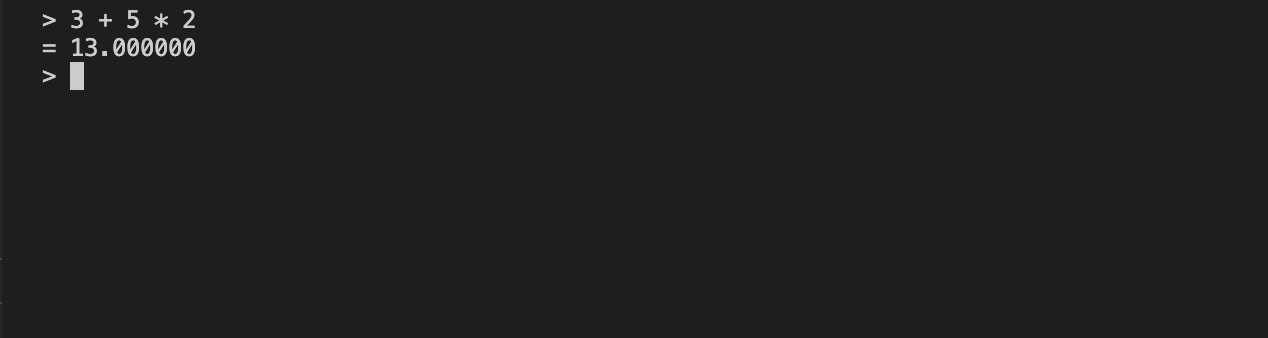
\includegraphics[scale=0.55]{naivetest.png}}
	\caption{Демонстрация работы программы}
	\label{pic6}
\end{figure}

\section{Сравнение полученных реализаций}

Проведём анализ производительности полученных версий анализатора. В качестве данных для тестирования возьмем выражения вида
$ \underbrace{2 + 2 + 2 \ldots + 2}_{n}$ для $ n = 1 \ldots 100$ с шагом $1$. Для вычисления времени выполнения воспользуемся библиотекой \texttt{time} Python 3.9.5. Автоматизацию обеспечим с помощью библиотеки \texttt{subprocess}. Получим следующий код:

\begin{minted}[linenos, breaklines=true, style=bw]{python}
import subprocess as sb
import time
import sys
def run(args):
    return sb.run(args,
        capture_output=True, ).stdout.decode().strip()
        
def main():
    if (len(sys.argv) < 6):
        print("Invalid arguments" )
        return
    exe_path = sys.argv[1]
    out_path = sys.argv[2]
    right_bound = int(sys.argv[3])
    step = int(sys.argv[4])
    iter = sys.argv[5]
    
    f = open(out_path, "w" )
    f.write(f " { exe_path} \n")
    f.close()
    for expr_len in range(1, right_bound, step):
	test_string = "+" .join(['2' ] * expr_len)
	args = [exe_path, test_string, iter]
	t = time.monotonic()
	run(args)
	end_t = time.monotonic()
	f = open(out_path, "a" )
	f.write(f " { expr_len} { (end_t - t) / (int(iter))} \n")
	f.close()
	print(f " Step { expr_len} finished" )

if __name__ == "__main__" :
    main()
\end{minted}

Кроме того, отметим, что в ранее написанные программы были внесены некоторые изменения для проведения эксперимента. Ознакомиться с ними можно в приложении \ref{appendA}.

Ознакомиться с полным исходным кодом программы, осуществляющей исследование производительности можно в приложении \ref{appendB}.

Для большей наглядности графики интерполированы полиномом с помощью функции \texttt{polyfit} библиотеки \texttt{numpy}.

Ознакомиться с полным исходным кодом программы, осуществляющей анализ полученных результатов можно в приложении \ref{appendC}.

Результаты исследования изображены на рис. \ref{pic7}:

\begin{figure}[H]
	\center{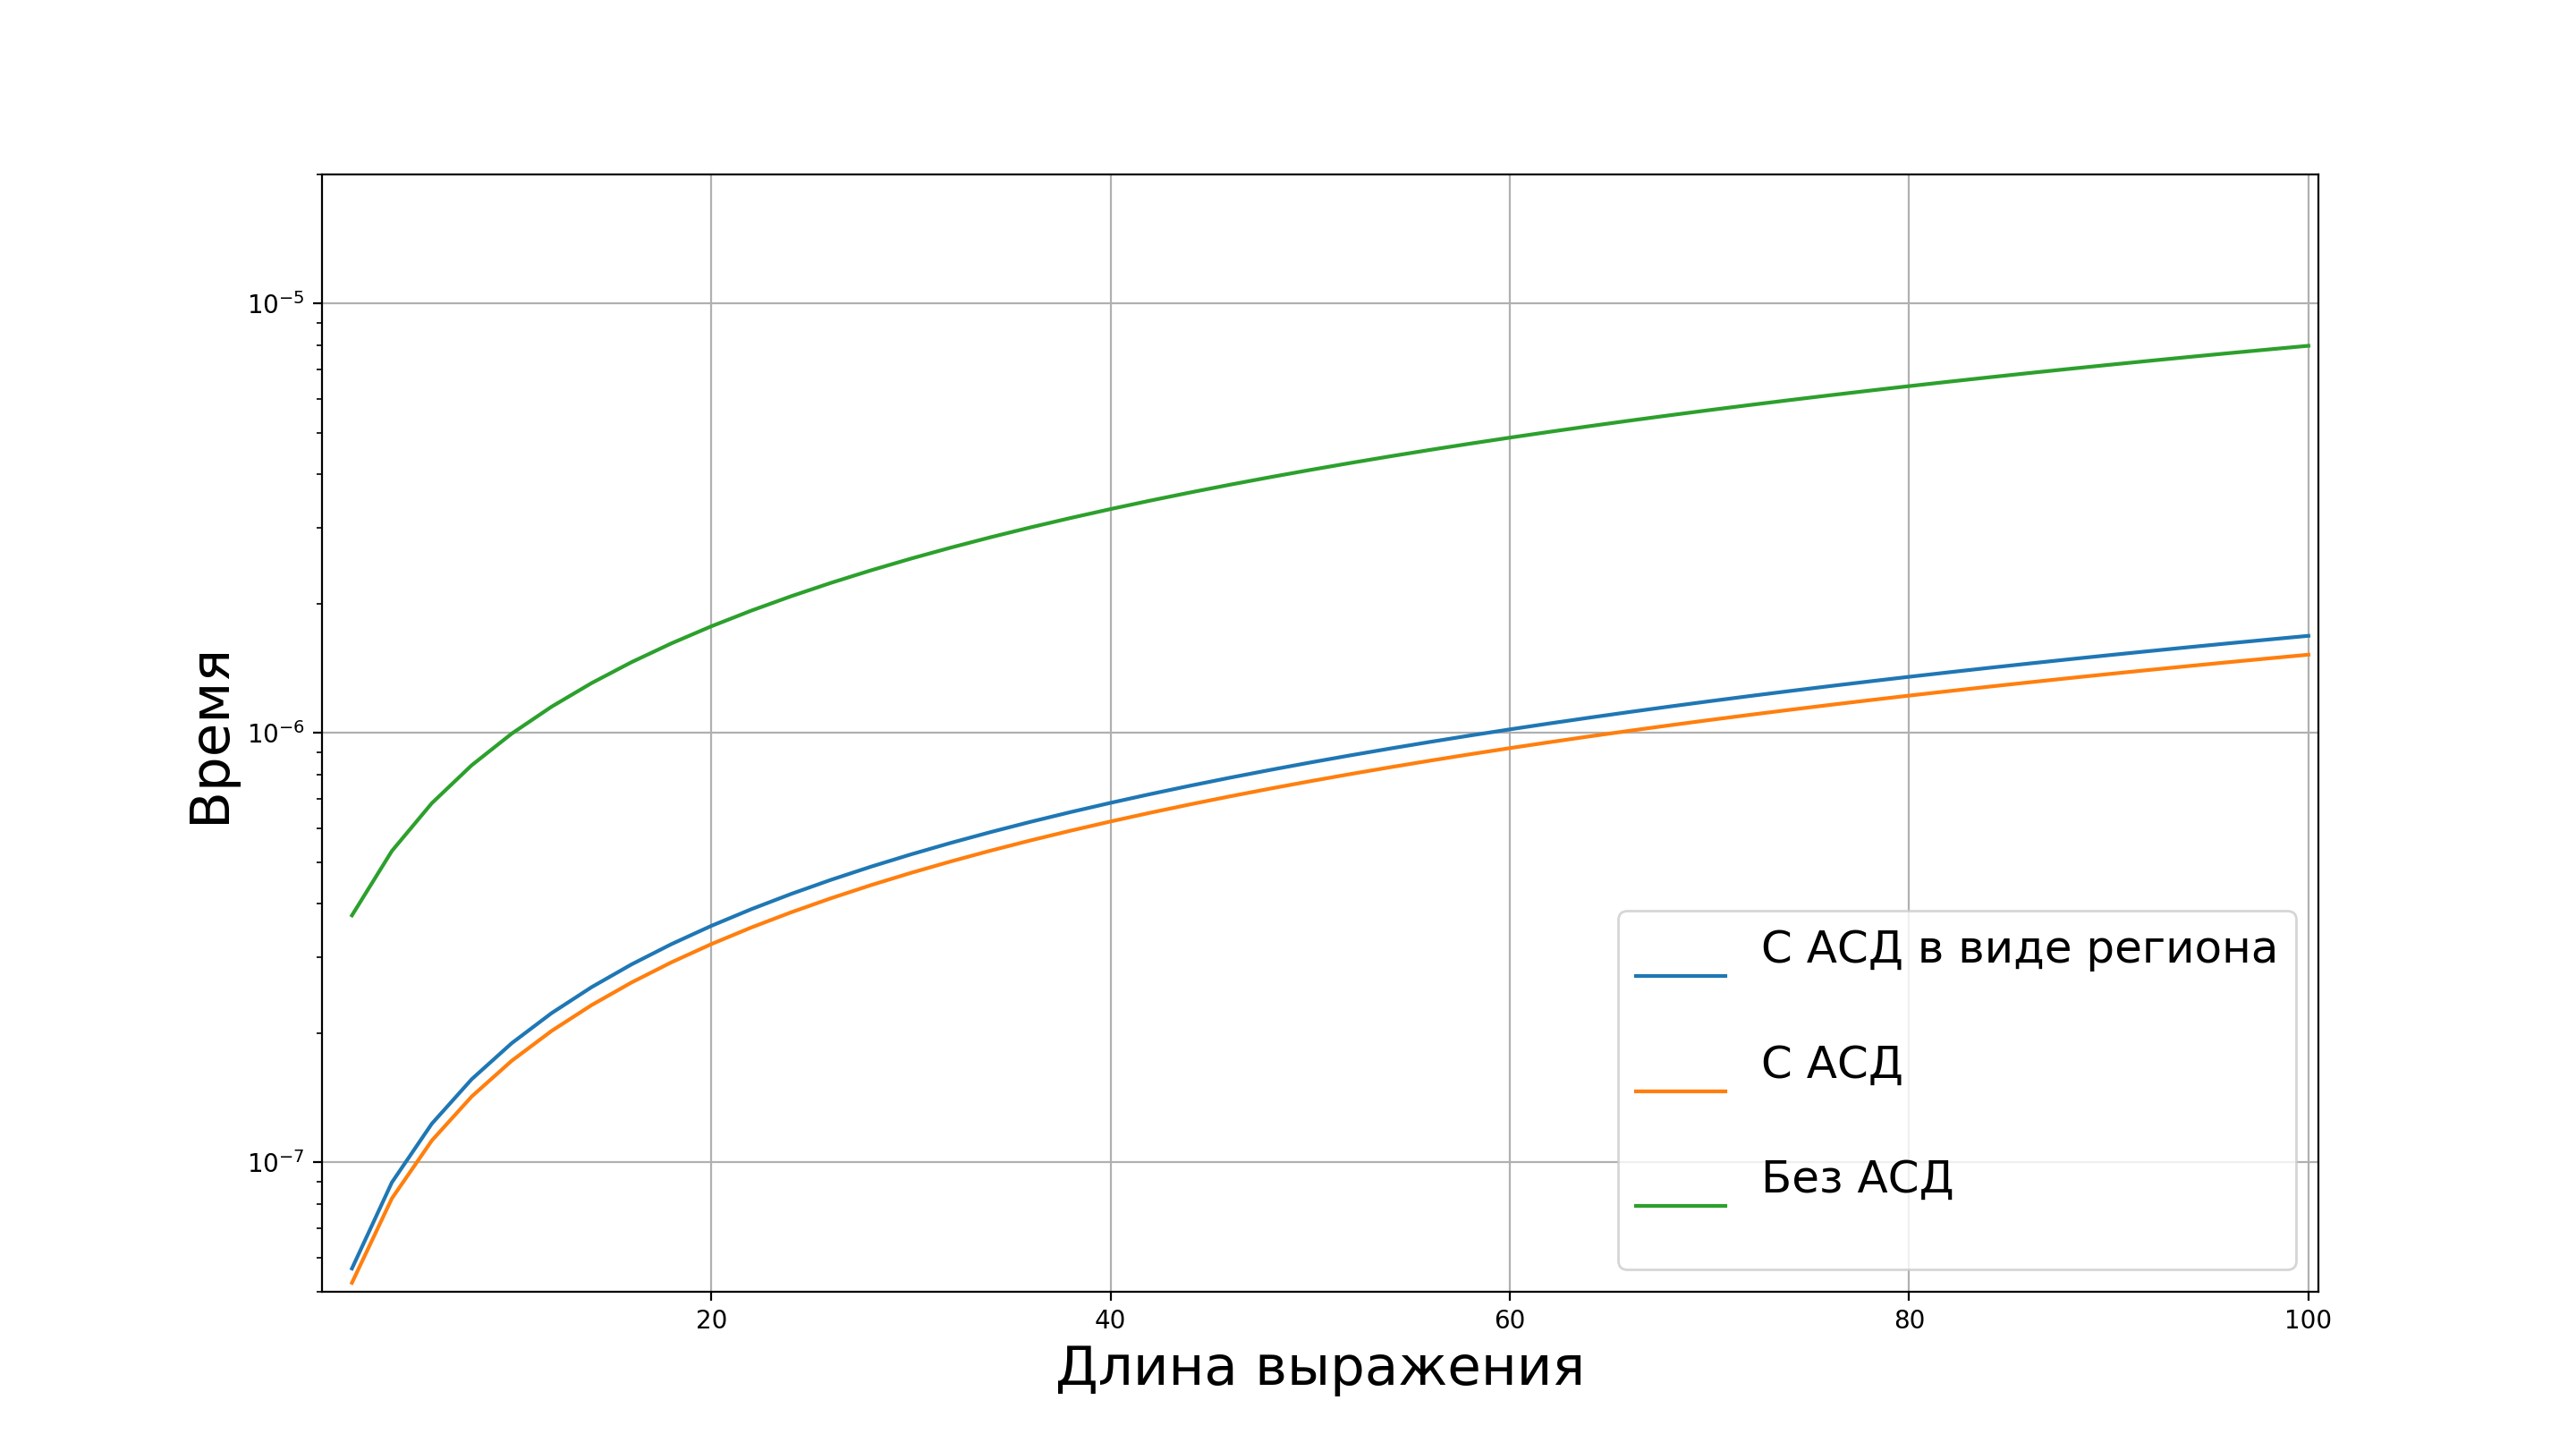
\includegraphics[scale=0.45]{benchmark.png}}
	\caption{Сравнение полученных результатов}
	\label{pic7}
\end{figure}

Исследование показало, что использование абстрактных синтаксических деревьев позволяет уменьшить время работы программы более чем в 5 раз, что существенно заметно для выражений любой длины.

Также из графиков видно, что в рамках данной работы не удалось добиться большей производительности при управлении памятью на основе регионов. Тем не менее, она все еще может считаться более предпочительной ввиду перечисленных ранее преимуществ.

% Раздел "Заключение"

\conclusion
В ходе данной работы:

\begin{enumerate}
	\item Были изучены теоретические основы построения лексических и синтаксических анализаторов.
	\item Проанализированы особенности реализации лексических и синтаксических анализаторов.
	\item Были изучены принципы работы генераторов лексического и синтаксического анализа на примере Flex и GNU Bison.
	\item Были созданы лексический и синтаксический анализаторы для анализа математического выражения.
	\item Было изучено понятие абстрактного синтаксического дерева.
	\item Проведен анализ производительности полученных реализаций.
\end{enumerate}

Таким образом, все поставленные в рамках работы задачи выполнены.

Результаты исследования показали, что абстрактные синтаксические деревья позволяют добиться увеличения производительности в 5–6 раз.

А это, в свою очередь, позволяет утверждать о том, что концепция абстрактных синтаксических деревьев является крайне важной в информатике и ее приложениях, в частности, при создании синтаксических анализаторов.

% Библиографический список, составленный вручную, без использования BibTeX
%
% \begin{thebibliography}{99}
%   \bibitem{Ione} Источник 1.
%   \bibitem{Itwo} Источник 2
% \end{thebibliography}

% Отобразить все источники. Даже те, на которые нет ссылок.
\nocite{*}

% Меняем inputencoding на лету, чтобы работать с библиографией в кодировке
% `cp1251', в то время как остальной документ находится в кодировке `utf8'
% Credit: Никита Рыданов
\inputencoding{cp1251}
\bibliographystyle{gost780uv}
\bibliography{thesis}
\inputencoding{utf8}

% При использовании biblatex вместо bibtex
% \printbibliography

% Окончание основного документа и начало приложений Каждая последующая секция
% документа будет являться приложением
\appendix

\section{Приложение A}
\label{appendA}
\begin{center}
\textbf{Flash-носитель с исходным кодом программ, использующихся в работе}
\end{center}
\textbf{Папка} \texttt{src} содержит оригинальный исходный код программы:
\begin{description}
	\item \textbf{Папка} \texttt{naive} — реализация без АСД
	\item \textbf{Папка} \texttt{naiveast} — реализация с АСД
	\item \textbf{Папка} \texttt{arena} — реализация с АСД на основе региона
\end{description}
\textbf{Папка} \texttt{extsrc} содержит измененный исходный код, необходимый для исследования производительности:
\begin{description}
	\item \textbf{Папка} \texttt{naive} — реализация без АСД
	\item \textbf{Папка} \texttt{naiveast} — реализация с АСД
	\item \textbf{Папка} \texttt{arena} — реализация с АСД на основе региона
\end{description}
%\includepdf[pages=-]{indtask_1.pdf}

\section{Приложение Б}
\label{appendB}
\begin{center}
\textbf{Исходный код программы на Python, осуществляющей исследование производительности полученных реализаций}
\end{center}

\begin{minted}[linenos, breaklines=true, style=bw]{python}
import subprocess as sb
import time
import sys
def run(args):
    return sb.run(args,
	capture_output=True, ).stdout.decode().strip()
	
def main():
    if (len(sys.argv) < 6):
	print("Invalid arguments" )
	return
    exe_path = sys.argv[1]
    out_path = sys.argv[2]
    right_bound = int(sys.argv[3])
    step = int(sys.argv[4])
    iter = sys.argv[5]

    f = open(out_path, "w" )
    f.write(f"{exe_path} \n " )
    f.close()
    for expr_len in range(1, right_bound, step):
	test_string = "+" .join(['2' ] * expr_len)
	args = [exe_path, test_string, iter]
	t = time.monotonic()
	run(args)
	end_t = time.monotonic()
	f = open(out_path, "a" )
	f.write(f"{expr_len} {(end_t - t) / (int(iter))} \n " )
	f.close()
	print(f" Step {expr_len} finished" )

if __name__ == "__main__" :
    main()
\end{minted}

\section{Приложение В}
\label{appendC}
\begin{center}
\textbf{Исходный код программы на Python, осуществляющей анализ полученных результатов}
\end{center}

\begin{minted}[linenos, breaklines=true, style=bw]{python}
import subprocess as sb
from time import time
import matplotlib.pyplot as plt
import sys
import numpy as np

legend = []
for index in range(1, len(sys.argv)):
    file_name = sys.argv[index]
    f = open(file_name, "r" )
    try:
	parser_type = f.readline()
    except StopIteration:
	parser_type = "Undefined parser"
    legend.append(parser_type)

    x_axis = []
    y_axis = []
    for line in f:
	try:
	    w, h = [float(x) for x in next(f).split()]
	except StopIteration:
	    break
	x_axis.append(w)
	y_axis.append(h)
    plt.xlabel("Длина выражения" , size = 22)
    plt.ylabel("Время" , size = 22)
    p = np.polyfit(x_axis, y_axis, 1)
    for i in range(len(x_axis)):
	y_axis[i] = p[0] * x_axis[i] + p[1]
    plt.plot(x_axis, y_axis)
plt.xlim(0.5, 100.5)
plt.ylim(5e-8, 2e-5)
plt.rcParams.update({'font.size': 18})
#plt.yscale("log")
plt.grid(True)
plt.legend(legend, loc="lower right" )
plt.show()
\end{minted}

\end{document}
